\chapter{Trattazione teorica estesa}
\captionsetup[figure]{font=small,labelfont=bf}
\label{app:teoria}

\section{Fondamenti del calcolo quantistico}
\label{app:fondamenti}
\begin{onehalfspace}

Questa sezione sviluppa in forma estesa i richiami di meccanica quantistica che la
Sezione~\ref{chap:fondamenti} del Capitolo~\ref{chap:shor} usa nella misura
minima necessaria a seguire l'algoritmo.

\subsection{Dalla Meccanica Classica alla Meccanica Quantistica}

La meccanica quantistica descrive il comportamento della materia e dell'energia alle scale atomiche e subatomiche, dove i principi della fisica classica cessano di essere validi. I suoi postulati, formulati nella prima metà del Novecento da Heisenberg, Schrödinger, Dirac e Bohr, introducono concetti radicalmente diversi da quelli classici: lo stato di un sistema fisico non è determinato in modo assoluto, ma è descritto da una \textbf{funzione d'onda} la cui evoluzione è governata dall'equazione di Schrödinger.

Il calcolo quantistico traduce questi principi fisici in risorse computazionali. La \textbf{sovrapposizione} consente a un bit quantistico di trovarsi in una combinazione lineare di 0 e 1 simultaneamente; l'\textbf{entanglement} crea correlazioni non classiche tra qubit distinti; l'\textbf{interferenza} permette di amplificare le soluzioni corrette e cancellare quelle errate.

\clearpage
\subsection{I Postulati della Meccanica Quantistica}

Il formalismo matematico della meccanica quantistica poggia su quattro postulati fondamentali, che costituiscono l'assiomatica della teoria e il punto di partenza rigoroso per la descrizione di qualsiasi sistema quantistico \cite{nielsenChuang2000}.

\begin{enumerate}
    \item \textbf{Postulato dello spazio degli stati.} Ad ogni sistema fisico isolato è associato uno \textbf{spazio di Hilbert} $\mathcal{H}$, detto \textit{spazio degli stati} del sistema. Lo stato del sistema è completamente descritto da un vettore unitario $\ket{\psi} \in \mathcal{H}$, detto \textit{vettore di stato} o \textit{ket}. Per un sistema a due livelli (qubit), $\mathcal{H} = \mathbb{C}^2$ e lo stato generale è $\ket{\psi} = \alpha\ket{0} + \beta\ket{1}$ con $|\alpha|^2 + |\beta|^2 = 1$.

    \item \textbf{Postulato dell'evoluzione.} L'evoluzione di un sistema quantistico chiuso è descritta da una \textbf{trasformazione unitaria}: se lo stato del sistema all'istante $t_1$ è $\ket{\psi(t_1)}$, allora all'istante $t_2$ esso si trova nello stato
    \begin{equation}
        \ket{\psi(t_2)} = U(t_1, t_2)\ket{\psi(t_1)}
    \end{equation}
    dove $U(t_1, t_2)$ è un operatore unitario ($U^\dagger U = I$) che dipende dagli istanti $t_1$ e $t_2$. In forma differenziale, l'evoluzione è governata dall'\textbf{equazione di Schrödinger}:
    \begin{equation}
        i\hbar \frac{d}{dt}\ket{\psi(t)} = \hat{H}\ket{\psi(t)}
    \end{equation}
    dove $\hat{H}$ è l'\textbf{Hamiltoniano} del sistema --- un operatore hermitiano ($\hat{H} = \hat{H}^\dagger$) che rappresenta l'energia totale --- e $\hbar = h/(2\pi)$ è la costante di Planck ridotta.\footnote{Nel calcolo quantistico a porte, ogni porta è la realizzazione discreta di questo postulato: la matrice unitaria $U$ descrive l'evoluzione del registro di qubit in un passo computazionale. L'Hamiltoniano fisico che implementa una porta specifica dipende dall'architettura hardware (impulsi a microonde per qubit superconduttori, impulsi laser per ioni intrappolati, ecc.).}

    \item \textbf{Postulato della misura.} Le misure quantistiche sono descritte da un insieme $\{M_m\}$ di \textbf{operatori di misura}, indicizzati dagli esiti $m$, soggetti alla relazione di completezza:
    \begin{equation}
        \sum_m M_m^\dagger M_m = I
    \end{equation}
    Se il sistema si trova nello stato $\ket{\psi}$ prima della misura, la probabilità di ottenere l'esito $m$ è:
    \begin{equation}
        p(m) = \bra{\psi} M_m^\dagger M_m \ket{\psi}
    \end{equation}
    e lo stato immediatamente dopo la misura con esito $m$ è il vettore normalizzato:
    \begin{equation}
        \ket{\psi'} = \frac{M_m\ket{\psi}}{\sqrt{p(m)}}
    \end{equation}
    Nel caso della \textbf{misura proiettiva in base computazionale} --- il caso standard nel calcolo quantistico --- gli operatori sono i proiettori $M_m = \ket{m}\bra{m}$, e la probabilità di ottenere $m$ si riduce alla \textbf{regola di Born}: $p(m) = |\braket{m|\psi}|^2$. La misura è un'operazione \textit{non unitaria} e \textit{irreversibile}: il collasso dello stato distrugge irrecuperabilmente le ampiezze che non corrispondono all'esito osservato.

    \item \textbf{Postulato dei sistemi composti.} Lo spazio degli stati di un sistema fisico composto da $n$ sottosistemi con spazi $\mathcal{H}_1, \ldots, \mathcal{H}_n$ è il \textbf{prodotto tensoriale}:
    \begin{equation}
        \mathcal{H} = \mathcal{H}_1 \otimes \mathcal{H}_2 \otimes \cdots \otimes \mathcal{H}_n
    \end{equation}
    Se ciascun sottosistema $i$ si trova nello stato $\ket{\psi_i}$, lo stato del sistema composto è $\ket{\psi_1} \otimes \ket{\psi_2} \otimes \cdots \otimes \ket{\psi_n}$. Esistono tuttavia stati del sistema composto --- gli stati \textbf{entangled} --- che non possono essere scritti in questa forma fattorizzata per nessuna scelta degli stati individuali: gli esiti delle misure sui due sottosistemi risultano correlati, indipendentemente dalla distanza fisica tra i due.
\end{enumerate}

Questi quattro postulati forniscono il quadro assiomatico completo entro cui si collocano tutti i concetti che seguono: il qubit (Postulato~1), le porte quantistiche come trasformazioni unitarie (Postulato~2), la misura e il collasso dello stato (Postulato~3), i registri multi-qubit e l'entanglement (Postulato~4).

\clearpage
\subsection{Il Qubit}

\subsubsection{Definizione Matematica}

L'unità fondamentale del calcolo quantistico è il \textbf{qubit} (\textit{quantum bit}). Mentre un bit classico assume uno dei due valori $\{0, 1\}$, un qubit è descritto da un vettore unitario nello spazio di Hilbert bidimensionale $\mathcal{H} = \mathbb{C}^2$, cioè uno spazio vettoriale complesso dotato di prodotto interno.

Nella \textbf{notazione di Dirac}, in cui $\ket{\psi}$ è detto \textit{ket}, $\bra{\psi}$ \textit{bra} e il prodotto interno $\braket{\phi|\psi}$ \textit{bracket}, i due stati base computazionali sono:
\begin{equation}
    \ket{0} = \begin{pmatrix} 1 \\ 0 \end{pmatrix}, \qquad
    \ket{1} = \begin{pmatrix} 0 \\ 1 \end{pmatrix}
\end{equation}

Lo stato generico di un qubit è la \textbf{sovrapposizione}:
\begin{equation}
    \ket{\psi} = \alpha\ket{0} + \beta\ket{1}, \qquad \alpha, \beta \in \mathbb{C}, \quad |\alpha|^2 + |\beta|^2 = 1
\end{equation}

dove $|\alpha|^2$ e $|\beta|^2$ rappresentano le probabilità di ottenere rispettivamente $0$ e $1$ al momento della misura. Il vincolo di normalizzazione $|\alpha|^2 + |\beta|^2 = 1$ garantisce che le probabilità sommino a 1.

\subsubsection{La Sfera di Bloch}

Ogni stato puro di un qubit può essere visualizzato come un punto sulla superficie della \textbf{sfera di Bloch}, una sfera unitaria in $\mathbb{R}^3$. Parametrizzando le ampiezze complesse tramite angoli reali $\theta \in [0, \pi]$ e $\phi \in [0, 2\pi)$:
\begin{equation}
    \ket{\psi} = \cos\!\left(\frac{\theta}{2}\right)\ket{0} + e^{i\phi}\sin\!\left(\frac{\theta}{2}\right)\ket{1}
\end{equation}

I poli nord e sud corrispondono agli stati $\ket{0}$ e $\ket{1}$, mentre i punti sull'equatore rappresentano sovrapposizioni equiprobabili con fasi diverse.

\subsection{Sistemi Multi-Qubit e Prodotto Tensoriale}

Un sistema di $n$ qubit è descritto da un vettore nello spazio di Hilbert $\mathcal{H}^{\otimes n} = \mathbb{C}^{2^n}$, ottenuto come prodotto tensoriale degli spazi individuali. Uno stato generico di $n$ qubit è:
\begin{equation}
    \ket{\psi} = \sum_{x \in \{0,1\}^n} \alpha_x \ket{x}, \qquad \sum_{x} |\alpha_x|^2 = 1
\end{equation}

La dimensione esponenziale $2^n$ dello spazio di Hilbert rende disponibili
ampiezze e correlazioni che non compaiono in un registro classico di $n$ bit:
con $n = 300$ qubit, lo spazio degli stati ha dimensione $2^{300}$, superiore
al numero di atomi nell'universo osservabile. Questa dimensione, tuttavia, non
implica da sola un vantaggio computazionale: esistono famiglie di stati e
circuiti quantistici descrivibili classicamente in modo efficiente. Il vantaggio
richiede che preparazione, interferenza e misura sfruttino la struttura del
problema, come avviene nel period finding di Shor.

\subsubsection{Entanglement}

Due qubit sono detti \textbf{entangled} quando il loro stato congiunto non può essere scritto come prodotto tensoriale degli stati individuali. Gli stati di Bell costituiscono la base canonica degli stati entangled a due qubit:
\begin{align}
    \ket{\Phi^+} &= \frac{1}{\sqrt{2}}(\ket{00} + \ket{11}) \\
    \ket{\Phi^-} &= \frac{1}{\sqrt{2}}(\ket{00} - \ket{11}) \\
    \ket{\Psi^+} &= \frac{1}{\sqrt{2}}(\ket{01} + \ket{10}) \\
    \ket{\Psi^-} &= \frac{1}{\sqrt{2}}(\ket{01} - \ket{10})
\end{align}

Lo stato $\ket{\Phi^+}$ non può essere fattorizzato come $\ket{\psi_A} \otimes \ket{\psi_B}$ per nessuna scelta di $\ket{\psi_A}$ e $\ket{\psi_B}$: misurare il primo qubit come $0$ garantisce che il secondo, misurato nella stessa base, dia anch'esso $0$, indipendentemente dalla distanza fisica tra i due sistemi. La correlazione non consente però di trasmettere informazione: le statistiche locali del secondo qubit non dipendono da ciò che si misura sul primo. Con opportune scelte delle basi di misura, gli stati entangled violano le disuguaglianze di Bell e producono correlazioni incompatibili con modelli a variabili nascoste locali~\cite{bell1964,aspect1982}.

Il circuito di preparazione si ottiene applicando Hadamard al primo qubit e
una CNOT fra i due qubit.

\subsubsection{L'Entanglement come Risorsa Fisica Fragile}
\label{sec:entanglement_fragile}

L'entanglement non è soltanto una proprietà astratta degli stati quantistici: è la \textbf{risorsa fisica} che gli algoritmi quantistici consumano per ottenere il loro vantaggio computazionale. Nell'algoritmo di Shor, il registro di controllo e il registro di lavoro devono restare entangled per tutta la durata della phase estimation affinché la Quantum Fourier Transform possa estrarre il periodo corretto. La perdita anche parziale di questa correlazione è sufficiente a degradare il risultato.

La fragilitá dell'entanglement ha un'origine fisica precisa. Un sistema quantistico reale non è mai perfettamente isolato dall'ambiente che lo circonda: campi elettromagnetici residui, vibrazioni termiche del reticolo cristallino e fluttuazioni di carica si accoppiano continuamente ai qubit. Quando questo accoppiamento avviene, il sistema entra in uno stato entangled \textit{con l'ambiente}, trasferendo ad esso parte dell'informazione di fase. Dal punto di vista del solo sistema, le ampiezze di interferenza si riducono: il qubit non è più in una sovrapposizione pura $\alpha\ket{0}+\beta\ket{1}$, ma in un \textbf{miscuglio statistico} in cui la fase relativa tra $\ket{0}$ e $\ket{1}$ è persa. Questo processo prende il nome di \textbf{decoerenza}~\cite{zurek2003}.

Il tempo caratteristico entro cui questa perdita di fase diventa apprezzabile è $T_2$, il \textbf{tempo di coerenza di fase} (\textit{dephasing time}). Esso misura per quanto tempo un qubit riesce a mantenere la propria sovrapposizione coerente prima che l'interazione con l'ambiente la degradi. La trattazione quantitativa è nella Sezione~\ref{app:fonti_fisiche_estese}.

\subsection{Porte Quantistiche}

Le operazioni su qubit sono rappresentate da \textbf{matrici unitarie}: $U^\dagger U = I$. La condizione di unitarietà garantisce la reversibilità del calcolo e la conservazione della norma (delle probabilità).

\subsubsection{Porte a Singolo Qubit}

Le tre \textbf{matrici di Pauli} $X$, $Y$, $Z$ costituiscono una base per lo spazio delle matrici $2\times 2$ hermitiane a traccia nulla; aggiungendo l'identità $I$ si ottiene una base di tutte le matrici hermitiane $2\times 2$. Giocano un ruolo centrale sia nella descrizione degli stati del qubit sia nella caratterizzazione dei canali di rumore.

\textbf{Porta di Pauli-X (NOT quantistico / Bit Flip):}
\begin{equation}
    X = \begin{pmatrix} 0 & 1 \\ 1 & 0 \end{pmatrix}, \qquad X\ket{0} = \ket{1}, \quad X\ket{1} = \ket{0}
\end{equation}
È l'analogo quantistico del NOT classico: inverte i valori di $\ket{0}$ e $\ket{1}$.

\textbf{Porta di Pauli-Y:}
\begin{equation}
    Y = \begin{pmatrix} 0 & -i \\ i & 0 \end{pmatrix}, \qquad Y\ket{0} = i\ket{1}, \quad Y\ket{1} = -i\ket{0}
\end{equation}
Combina un bit flip e un phase flip: è equivalente (a meno di una fase globale) alla composizione $iXZ$. Compare naturalmente nella decomposizione di rotazioni generali su qubit e nella descrizione del canale di \textit{depolarizzazione}.

\textbf{Porta di Pauli-Z (Phase Flip):}
\begin{equation}
    Z = \begin{pmatrix} 1 & 0 \\ 0 & -1 \end{pmatrix}, \qquad Z\ket{0} = \ket{0}, \quad Z\ket{1} = -\ket{1}
\end{equation}
Lascia invariato $\ket{0}$ e aggiunge una fase $-1$ a $\ket{1}$: è un \textit{phase flip}.

Le tre matrici di Pauli soddisfano le seguenti relazioni algebriche fondamentali:
\begin{align}
    X^2 = Y^2 = Z^2 &= I \\
    XY = iZ, \quad YZ = iX, &\quad ZX = iY \\
    \{X, Y\} = \{Y, Z\} &= \{X, Z\} = 0
\end{align}
dove $\{A, B\} = AB + BA$ è l'\textbf{anticommutatore}. La seconda relazione riflette la struttura dell'algebra di Lie $\mathfrak{su}(2)$, generata da $iX/2$, $iY/2$, $iZ/2$; la terza --- l'anticommutazione --- è alla base della struttura dei codici di correzione degli errori quantistici, dove $X$ e $Z$ rappresentano rispettivamente errori di bit flip e phase flip indipendenti.

\textbf{Porta di Hadamard:}
\begin{align}
    H &= \frac{1}{\sqrt{2}}\begin{pmatrix} 1 & 1 \\ 1 & -1 \end{pmatrix} \notag \\[8pt]
    H\ket{0} &= \frac{\ket{0}+\ket{1}}{\sqrt{2}} \equiv \ket{+}, \qquad
    H\ket{1} = \frac{\ket{0}-\ket{1}}{\sqrt{2}} \equiv \ket{-}
\end{align}

La porta di Hadamard è fondamentale: applicata a $n$ qubit inizializzati in $\ket{0}^{\otimes n}$, genera la \textbf{sovrapposizione uniforme} di tutti i $2^n$ stati base:
\begin{equation}
    H^{\otimes n}\ket{0}^{\otimes n} = \frac{1}{\sqrt{2^n}}\sum_{x=0}^{2^n-1}\ket{x}
\end{equation}

\textbf{Porta di fase $R_\phi$:}
\begin{equation}
    R_\phi = \begin{pmatrix} 1 & 0 \\ 0 & e^{i\phi} \end{pmatrix}
\end{equation}
Casi particolari: $T = R_{\pi/4}$ (T-gate) e $S = R_{\pi/2}$ (S-gate o Phase gate).

\subsubsection{Porte a Due Qubit}

\textbf{Porta \ac{CNOT}:}
\begin{equation}
    \text{CNOT} = \begin{pmatrix} 1&0&0&0 \\ 0&1&0&0 \\ 0&0&0&1 \\ 0&0&1&0 \end{pmatrix}
\end{equation}
Applica una NOT sul qubit \textit{target} se e solo se il qubit \textit{control} è $\ket{1}$. È la porta a due qubit più comune e, insieme alle porte a singolo qubit, forma un insieme universale.

\textbf{Porta Toffoli (\ac{CCNOT}):} Generalizzazione a tre qubit; applica NOT sul terzo qubit solo se entrambi i qubit di controllo sono $\ket{1}$.

\begin{figure}[H]
    \centering
    \includegraphics[width=0.88\textwidth]{circuit_gates.png}

\caption[Porte quantistiche a singolo e due qubit]{Simboli circuitali delle principali porte quantistiche a singolo qubit ($X$, $Y$, $Z$, $H$, $R_\phi$) e della porta CNOT a due qubit. Nella porta CNOT, il punto pieno indica il qubit di controllo $q_c$ e il cerchio con croce indica il qubit target $q_t$.}\label{fig:gates}
\end{figure}
\clearpage
\subsection{Circuiti Quantistici}

Un \textbf{circuito quantistico} è una sequenza ordinata di porte quantistiche applicata a un registro di qubit. I circuiti si leggono da sinistra a destra, con ogni filo orizzontale che rappresenta l'evoluzione temporale di un qubit. La composizione di porte corrisponde al prodotto matriciale degli operatori unitari associati.

L'equivalente quantistico del teorema di universalità classico afferma che qualunque trasformazione unitaria su $n$ qubit può essere \textbf{approssimata con precisione arbitraria} da una sequenza finita di porte prese da un insieme universale, tipicamente $\{H, T, \text{CNOT}\}$. La distinzione fra approssimazione e decomposizione esatta non è pedanteria: le sequenze finite su un insieme di porte fissato sono numerabili, mentre le trasformazioni unitarie non lo sono, sicché una decomposizione esatta è impossibile in generale. Il teorema di Solovay--Kitaev garantisce che l'approssimazione a precisione $\varepsilon$ richiede $O(\log^c(1/\varepsilon))$ porte, con $c$ costante piccola: il costo dell'approssimazione cresce dunque solo polilogaritmicamente, ed è questa la ragione per cui l'universalità resta praticamente utile.

\subsection{Interferenza Quantistica}

Poiché la misura distrugge le ampiezze (Postulato~3), gli algoritmi quantistici devono amplificare la risposta corretta \emph{prima} della misura.

L'\textbf{interferenza} è il meccanismo fondamentale attraverso cui gli algoritmi quantistici realizzano il loro vantaggio computazionale. Le ampiezze quantistiche sono numeri complessi e possono combinarsi costruttivamente (quando hanno lo stesso segno/fase) o distruttivamente (quando hanno fase opposta).

Un algoritmo quantistico efficiente è costruito in modo che:
\begin{itemize}
    \item Le ampiezze degli stati \textbf{sbagliati} si cancellino per \textbf{interferenza distruttiva};
    \item Le ampiezze degli stati \textbf{corretti} si sommino per \textbf{interferenza costruttiva}.
\end{itemize}

Questo meccanismo è alla base sia dell'algoritmo di Grover sia dell'algoritmo di Shor (Capitolo~\ref{chap:shor}), dove la Quantum Fourier Transform realizza l'interferenza necessaria al ritrovamento del periodo.

\subsection{Modello di Complessità Quantistica}

La complessità di un algoritmo quantistico è misurata in termini di numero di porte (equivalente delle operazioni elementari classiche) e di profondità del circuito (numero di livelli di porte parallele). La classe centrale è \ac{BQP}, che contiene i problemi risolvibili da un computer quantistico in tempo polinomiale con probabilità di errore al più $1/3$.

Le inclusioni $\mathbf{P} \subseteq \mathbf{BPP} \subseteq \mathbf{BQP} \subseteq \mathbf{PSPACE}$ sono \emph{dimostrate}; ciò che resta aperto è se siano \textbf{strette}. Non è noto se BQP contenga propriamente P o BPP --- cioè se esista davvero un problema che un computer quantistico risolva efficientemente e uno classico no --- né se sia propriamente contenuto in PSPACE. Una dimostrazione di separazione stretta fra BQP e BPP implicherebbe $\mathbf{P} \neq \mathbf{PSPACE}$, un risultato che la teoria della complessità non ha ancora raggiunto: è questa la ragione per cui il vantaggio quantistico, per Shor come per gli altri algoritmi, resta una congettura ampiamente creduta e non un teorema.

\begin{figure}[H]
    \centering
    \includegraphics[width=0.68\textwidth]{complexity_classes.png}

\caption[Gerarchia delle classi di complessità quantistica]{Gerarchia delle classi di complessità nel calcolo quantistico. La classe BQP cattura i problemi efficientemente risolvibili da un computer quantistico; le inclusioni mostrate ($\mathrm{P} \subseteq \mathrm{BPP} \subseteq \mathrm{BQP} \subseteq \mathrm{PSPACE}$) sono dimostrate, mentre è congetturata --- e non dimostrata --- la loro \emph{strettezza}. Gli algoritmi di Shor e Grover risiedono in BQP; che la fattorizzazione non appartenga a P è ritenuto probabile ma non provato.}\label{fig:complexity}
\end{figure}

\end{onehalfspace}


\section{L'anatomia fisica di una QPU}
\label{app:anatomia}

Il Capitolo~\ref{chap:rumore} isola di questa materia i soli tre fatti che ricorrono nel
seguito; questa sezione ne d\`a la trattazione completa.

\subsection{Qubit, Controllo e Vincoli Fisici della QPU}

Per capire dove nascono gli errori bisogna prima capire com'è fatta la macchina. Una \ac{QPU} superconduttiva è un chip criogenico che contiene \emph{esclusivamente} i qubit e le linee fisiche che li collegano: contrariamente all'intuizione, \textbf{le porte logiche non risiedono nel chip}. Aprendo una CPU classica si trovano registri e porte logiche incise nel silicio; aprendo una QPU si trovano solo i qubit. Le operazioni sono realizzate dall'\textbf{elettronica di controllo esterna}, che invia impulsi a microonde convogliati ai qubit tramite guide d'onda: ``far passare un qubit in un gate'' significa in realtà inviargli un impulso sagomato che ne ruota lo stato sulla sfera di Bloch dell'angolo desiderato (90°, 30°, 10°, \ldots). La Figura~\ref{fig:qpu_anatomia} schematizza questa architettura per una QPU a 5 qubit con topologia a catena lineare.

\begin{figure}[H]
\centering
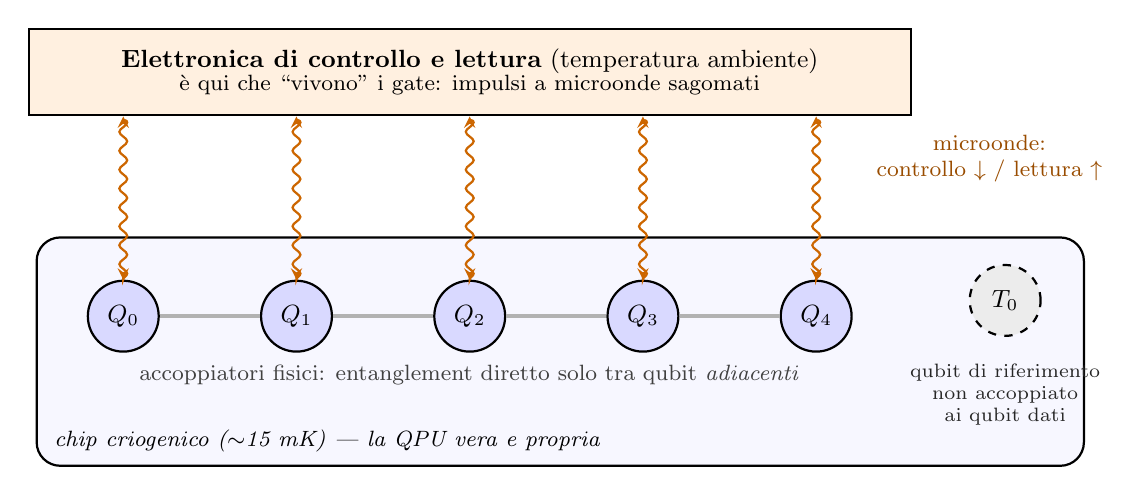
\begin{tikzpicture}[
  qubit/.style={circle, draw=black, thick, fill=blue!15, minimum size=9mm, font=\small},
  testq/.style={circle, draw=black, thick, dashed, fill=gray!15, minimum size=9mm, font=\small},
  wave/.style={decorate, decoration={snake, amplitude=0.5mm, segment length=2.4mm}, thick, <->, >=stealth, orange!80!black},
  coupl/.style={line width=1.6pt, gray!60}
]
\node[rectangle, draw=black, thick, fill=orange!12, minimum width=112mm, minimum height=11mm, align=center, font=\small] (E) at (4.4, 3.1)
  {\textbf{Elettronica di controllo e lettura} (temperatura ambiente)\\[-1mm] {\footnotesize è qui che ``vivono'' i gate: impulsi a microonde sagomati}};
\draw[rounded corners=3mm, thick, fill=blue!3] (-1.1,-1.9) rectangle (12.2,1.0);
\node[font=\footnotesize\itshape, anchor=south west] at (-1.0,-1.85) {chip criogenico ($\sim$15 mK) --- la QPU vera e propria};
\node[qubit] (Q0) at (0,0) {$Q_0$};
\node[qubit] (Q1) at (2.2,0) {$Q_1$};
\node[qubit] (Q2) at (4.4,0) {$Q_2$};
\node[qubit] (Q3) at (6.6,0) {$Q_3$};
\node[qubit] (Q4) at (8.8,0) {$Q_4$};
\draw[coupl] (Q0) -- (Q1);
\draw[coupl] (Q1) -- (Q2);
\draw[coupl] (Q2) -- (Q3);
\draw[coupl] (Q3) -- (Q4);
\node[font=\footnotesize, gray!50!black] at (4.4,-0.75) {accoppiatori fisici: entanglement diretto solo tra qubit \emph{adiacenti}};
\node[testq] (T0) at (11.2,0.2) {$T_0$};
\node[font=\scriptsize, align=center, gray!30!black] at (11.2,-1.0) {qubit di riferimento\\non accoppiato\\ai qubit dati};
\foreach \q in {Q0,Q1,Q2,Q3,Q4}{ \draw[wave] (E.south -| \q) -- (\q.north); }
\node[font=\footnotesize, orange!60!black, align=center] at (11.0,2.0) {microonde:\\controllo $\downarrow$ / lettura $\uparrow$};
\end{tikzpicture}

\caption[Anatomia schematica di una QPU superconduttiva a 5 qubit]{Schema didattico di una \ac{QPU} superconduttiva: cinque qubit in catena, qubit di riferimento $T_0$ ed elettronica esterna di controllo e lettura.}\label{fig:qpu_anatomia}
\end{figure}

Schema didattico di una \ac{QPU} superconduttiva a 5 qubit con topologia a catena. Nel chip criogenico risiedono qubit, risonatori e accoppiatori; le operazioni sono pilotate dall'elettronica esterna mediante linee di controllo e lettura. L'interazione a due qubit diretta è disponibile solo lungo gli accoppiamenti disegnati ($Q_1$--$Q_2$ sì, $Q_0$--$Q_2$ mediante routing). $T_0$ rappresenta un qubit di riferimento non accoppiato alla catena, ma ancora dotato delle linee necessarie a preparazione e misura: non fornisce una misura ``pura'' di $T_1$ e non elimina perdite, Purcell effect o altre sorgenti di decoerenza.


La Figura~\ref{fig:qpu_reale} mostra come questa architettura si presenta nella realtà: all'esterno il sistema integrato (criostato, elettronica e schermature racchiusi nella teca), all'interno della sala macchine i cilindri criogenici sospesi con il fascio di tubi e cavi coassiali che convogliano le microonde di controllo e lettura --- le ``guide d'onda'' dello schema precedente.

\begin{figure}[!htbp]
\centering
\subfloat[IBM Quantum System One]{\begin{minipage}{0.48\textwidth}\centering\includegraphics[width=\linewidth,height=36mm,keepaspectratio]{foto_system_one.jpg}\end{minipage}}\hfill
\subfloat[Criostati e cablaggio]{\begin{minipage}{0.48\textwidth}\centering\includegraphics[width=\linewidth,height=36mm,keepaspectratio]{foto_criostato_ibm.jpg}\end{minipage}}

\caption[La QPU reale: sistema integrato e criostati con cablaggio]{IBM Quantum System One (a) e criostati IBM Q con cablaggio di controllo (b). Crediti: IBM Research, CC~BY~2.0 (a); Connie Zhou per IBM, pubblico dominio (b), via Wikimedia Commons.}\label{fig:qpu_reale}
\end{figure}

La \ac{QPU} reale. (a)~Il sistema integrato IBM Quantum System One: il cilindro nero al centro è il criostato che contiene il chip, circondato dall'elettronica di controllo. (b)~Criostati IBM Q in sala macchine: dall'alto arrivano i tubi per la refrigerazione e i cavi coassiali che convogliano le microonde di controllo e lettura verso il chip, sospeso sul fondo del cilindro a $\sim$15\,mK.


\begin{figure}[!htbp]
\centering
\includegraphics[width=0.48\textwidth,height=0.25\textheight,keepaspectratio]{foto_chip_transmon.png}

\caption[Chip quantistico superconduttivo a 6 transmon con giunzioni di test]{Resa tridimensionale di un chip a sei transmon e dodici giunzioni di test. Credito: Onri Jay Benally, CC~BY~4.0, via Wikimedia Commons.}\label{fig:chip_transmon}
\end{figure}

Resa tridimensionale di un chip quantistico superconduttivo con 6 qubit transmon e 12 giunzioni di test. Si riconoscono gli elementi dello schema di Figura~\ref{fig:qpu_anatomia}: i qubit con i loro risonatori, le linee di accoppiamento, le piazzole dorate per il collegamento alle guide d'onda e --- ai quattro angoli --- le strutture di test isolate, l'analogo reale del qubit $T_0$.


Questa architettura ha tre conseguenze dirette per gli errori.

\paragraph{La lettura distrugge lo stato - fisicamente.}
Anche la misura avviene tramite microonde: ogni qubit è accoppiato a un risonatore, si invia un impulso di sonda al risonatore e se ne osserva la risposta, che cambia a seconda che il qubit sia in $\ket{0}$ o in $\ket{1}$ (lettura dispersiva). L'interazione con la sonda fa collassare lo stato del qubit misurato: il collasso del Postulato~3 è un processo fisico, non soltanto una regola matematica. Il segnale di lettura può inoltre disturbare i qubit vicini; per questo le misure a metà circuito richiedono calibrazioni dedicate e, nei circuiti di questa tesi, tutte le misure sono collocate alla fine.

\paragraph{Il budget di operazioni: coerenza vs velocità dei gate.}
Le prestazioni di una QPU dipendono dal rapporto tra due tempi: quanto a lungo il qubit resta coerente e quanto dura una singola operazione. Con una finestra di coerenza di $100\,\mu$s e gate da $\sim$25\,ns, si eseguono $\sim$4\,000 operazioni; una macchina con coerenza superiore ma gate più lenti può eseguirne \emph{meno}. È il rapporto che conta, non il singolo parametro --- ed è questo rapporto a decidere se il circuito di Shor per una data istanza è fisicamente eseguibile. La Tabella~\ref{tab:tecnologie_qpu} confronta gli ordini di grandezza delle due principali tecnologie.

\begin{table}[H]
\centering

\small
\begin{tabularx}{\textwidth}{@{}lXX@{}}
\toprule
 & \textbf{Superconduttori (IBM, IQM, \ldots)} & \textbf{Ioni intrappolati (IonQ, Quantinuum, \ldots)} \\
\midrule
Tempo di coerenza          & $50$--$300\,\mu$s                      & da secondi a minuti \\
\addlinespace[0.3em]
Durata gate (1 qubit)      & $\sim$15--40\,ns                       & $\sim$1--100\,$\mu$s \\
\addlinespace[0.3em]
Durata gate (2 qubit)      & $\sim$60--500\,ns                      & $\sim$0.1--1\,ms \\
\addlinespace[0.3em]
Operazioni per finestra    & $\sim 10^{3}$--$10^{4}$                & $\sim 10^{3}$ \\
\addlinespace[0.3em]
Lettura                    & più esposta a errori e interferenze     & più stabile e affidabile \\
\addlinespace[0.3em]
Crosstalk                  & presente (accoppiamento capacitivo)     & ridotto \\
\addlinespace[0.3em]
Velocità di esecuzione     & molto alta                              & bassa (gate lenti) \\
\bottomrule
\end{tabularx}
\caption[Confronto tra tecnologie di QPU: superconduttori vs ioni intrappolati]{Ordini di grandezza indicativi delle due principali tecnologie di \ac{QPU}. La coerenza lunghissima degli ioni intrappolati non si traduce in più operazioni utili, perché i gate sono da $10^3$ a $10^4$ volte più lenti: il budget di operazioni per finestra di coerenza è simile, ma i superconduttori lo spendono molto più in fretta. Gli ioni sono invece più robusti su lettura e crosstalk.}\label{tab:tecnologie_qpu}

\end{table}

\paragraph{La durata del circuito conta.}
La perdita di coerenza si accumula con il tempo: per un decadimento esponenziale con costante $T$, la probabilità che il qubit abbia perso l'informazione dopo un tempo $t$ è $1-e^{-t/T}$, che cresce con continuità al crescere di $t$. Non esiste quindi una soglia netta oltre la quale il calcolo fallisce, ma un circuito che occupa una frazione rilevante di $\min(T_1,T_2)$, come quello di Shor, arriva alla misura con una probabilità d'errore elevata anche se la sua durata è formalmente inferiore ai tempi di coerenza.

\paragraph{La topologia decide chi parla con chi.}
Le QPU differiscono anche per geometria: catene lineari, griglie (heavy-hex di IBM), connettività completa. Su una catena, una porta fra qubit non adiacenti richiede di avvicinare l'informazione con porte SWAP attraverso i qubit intermedi: ogni SWAP costa tre porte a due qubit, e quindi tempo ed errori aggiuntivi. La topologia determina quindi sia \emph{quali} circuiti si possono mappare in modo efficiente, sia \emph{dove} il crosstalk colpirà. Questo aspetto --- insieme al fatto che i parametri di coerenza variano da qubit a qubit dello stesso chip --- è ripreso nel Capitolo~\ref{chap:surface}, dove la località delle interazioni sulla griglia è il fondamento architetturale del surface code.

\subsection{Le quattro fonti fisiche: parametri e modelli di misura}
\label{app:fonti_fisiche_estese}

Questa sottosezione completa la Sezione~\ref{sec:fonti_fisiche} con formule,
ordini di grandezza e limiti interpretativi.

\subsubsection{Decoerenza: rilassamento e perdita di fase}

La \textbf{decoerenza} nasce dall'interazione con campi elettromagnetici
parassiti, fononi e fluttuazioni termiche. Il \textbf{tempo di rilassamento}
$T_1$ descrive il decadimento spontaneo da $\ket{1}$ a $\ket{0}$ per
dissipazione energetica; su dispositivi superconduttori è tipicamente
dell'ordine di $50$--$500\,\mu$s. Il \textbf{tempo di dephasing} $T_2$
descrive invece la randomizzazione della fase relativa e combina rilassamento e
perdita pura di fase:
\begin{equation}
    \frac{1}{T_2}=\frac{1}{2T_1}+\frac{1}{T_\phi},
    \label{eq:T2_decomp}
\end{equation}
dove $T_\phi$ è il tempo di puro dephasing; vale $T_2\leq2T_1$ e sono comuni
ordini di grandezza di $50$--$200\,\mu$s.

Sul cammino critico, il criterio
\begin{equation}
    \tau_{\text{circuito}}\ll\min(T_1,T_2)
\end{equation}
è soltanto euristico. La crescita polinomiale dell'aritmetica non determina una
soglia universale in bit: compilazione, parallelismo, idle, topologia e QEC
fissano la durata fisica effettiva. In particolare, durante la phase estimation
la coerenza di fase deve sostenere l'entanglement fra i registri; confrontare
$T_2/\tau_{\text{gate}}$ con il numero totale di porte sarebbe scorretto perché
un conteggio non è una durata. Per questo il noise model usa durate esplicite e
riporta separatamente conteggi e profondità.

\subsubsection{Errori di gate}

Un gate fisico realizza $\widetilde U=U+\delta E$ anziché $U$. Una misura
ideale della discrepanza è la gate infidelity
\begin{equation}
 r(U,\widetilde U)=1-F(U,\widetilde U),\qquad
 F(U,\widetilde U)=\frac{1}{d^2}
 \left|\operatorname{Tr}(U^\dagger\widetilde U)\right|^2.
\end{equation}
Le cause includono errori di ampiezza o frequenza degli impulsi, accoppiamento
\emph{always-on} e leakage verso livelli non computazionali
($\ket{2},\ket{3},\ldots$). Gli ordini indicativi 2024--2025 sono
$r\simeq0.03$--$0.1\%$ per gate 1Q e $0.3$--$1\%$ per gate 2Q; non sono
assunti come calibrazione delle campagne di questa tesi.

\subsubsection{Readout e crosstalk}

Il readout è descritto da una matrice di confusione
\begin{equation}
 A_{ij}=P(\text{misura }i\mid\text{stato }j),\qquad
 \sum_iA_{ij}=1.
\end{equation}
Sotto l'ipotesi d'indipendenza, per $n$ qubit vale
$A=\bigotimes_{k=1}^nA_k$, con
\begin{equation}
 A_k=\begin{pmatrix}
 1-e_0^{(k)}&e_1^{(k)}\\ e_0^{(k)}&1-e_1^{(k)}
 \end{pmatrix},
\end{equation}
dove $e_0^{(k)}$ è la probabilità di leggere $1$ dato $\ket{0}$; valori
indicativi sono $1$--$3\%$.

Il \textbf{crosstalk} è invece l'interferenza fra operazioni simultanee su
qubit vicini, dovuta soprattutto all'accoppiamento capacitivo residuo. Produce
rotazioni parassite, dipende dalla topologia ed è difficile da modellare
analiticamente~\cite{sarovar2020}. Proprio le correlazioni spaziali non
rappresentate nel grafo del decoder costituiscono, nella
Sezione~\ref{sec:decodifica_appresa}, il regime in cui il correttore residuo
appreso mostra un guadagno rispetto al riferimento analitico.


\section{L'algoritmo di Shor - approfondimenti e stato dell'arte}
\label{app:shor_esteso}

Questa sezione approfondisce l'algoritmo di Shor presentato nel Capitolo~\ref{chap:shor}: lo stato delle realizzazioni sperimentali, i miglioramenti algoritmici recenti, la sensibilità delle sue componenti al rumore e il perimetro delle istanze studiate.

\subsection{Sviluppi Recenti e Stato dell'Arte}

\subsubsection{Implementazioni su Hardware Reale}

Nonostante la solidità teorica, l'esecuzione di Shor su hardware reale rimane limitata a istanze molto piccole a causa dei requisiti di profondità circuitale. I principali risultati sperimentali sono:

\begin{itemize}
    \item \textbf{2001 -- \ac{NMR} (Vandersypen et al.)}: prima dimostrazione sperimentale di Shor su un sistema a 7 spin nucleari; fattorizzazione di $N = 15$ in $3 \times 5$ \cite{vandersypen2001}.
    \item \textbf{2016 -- Ioni intrappolati (Monz et al.)}: implementazione scalabile su 5 qubit ionici; fattorizzazione di $N = 15$ con un'architettura modulare \cite{monz2016}.
    \item \textbf{2021 -- Qubit superconduttori \ac{IBM}}: dimostrazione compilata della fattorizzazione di $N = 21$ su processori \ac{IBM} Quantum utilizzando 5 qubit \cite{skosana2021}.
\end{itemize}

Queste istanze evidenziano quanto la distanza dalle chiavi crittograficamente rilevanti sia ancora enorme. Una stima classica del fabbisogno, formulata sul modello di circuito privo di correzione d'errore, riporta $5K+1$ qubit di memoria e circa $72K^3$ gate elementari per fattorizzare un numero di $K$ bit \cite{beckman1996}; costanti e overhead dipendono però dall'architettura aritmetica e, nelle stime moderne, dal protocollo fault-tolerant, rispetto al quale quel conteggio va inteso come limite inferiore ottimistico. In ogni caso, i valori per RSA-2048 restano fuori portata per i processori \ac{NISQ} attuali.

Alla distanza teorica se ne aggiunge una operativa, documentata da una campagna recente su più piattaforme cloud: le costruzioni circuitali restano specifiche per ciascun modulo, e le fedeltà delle macchine si presentano instabili, con tassi d'errore elevati e fluttuanti \cite{shor_challenges2025}. È la ragione per cui, in questo lavoro, $N=15$ è trattato come istanza illustrativa e non come misura di fattibilità.

\subsubsection{Miglioramenti Algoritmici: Regev 2023}

Un risultato teorico rilevante è stato pubblicato nel 2023 da Oded Regev \cite{regev2023}. La proposta fattorizza un intero di $n$ bit eseguendo indipendentemente circa $\sqrt n+4$ circuiti, ciascuno con $\widetilde O(n^{3/2})$ gate, seguiti da post-processing classico polinomiale. Il confronto con Shor non può quindi essere ridotto al solo conteggio di gate di una singola esecuzione: aumentano il numero di run e, nella costruzione originale, anche lo spazio quantistico; inoltre l'articolo dichiara non chiaro l'effettivo vantaggio implementativo. Il risultato è un miglioramento asintotico importante, non una dimostrazione di praticabilità su dispositivi NISQ.

\subsection{Sensibilità delle componenti di Shor al rumore}
\label{app:shor_rumore_esteso}

La seguente analisi completa la parte sul rumore del Capitolo~\ref{chap:quadro}
con derivazioni, esempio numerico e figura di scala.

\subsubsection{Errori nella Quantum Fourier Transform}

La \ac{QFT} usa rotazioni
$R_k=\operatorname{diag}(1,e^{2\pi i/2^k})$ con angoli esponenzialmente
piccoli. Per $k=10$, $2\pi/1024\simeq6\times10^{-3}$ rad. Gli errori coerenti
di calibrazione possono sommarsi in ampiezza, mentre il canale depolarizzante
produce degradazione stocastica: non è quindi corretto ricondurli a un solo
``errore di fase'' lineare. Le campagne li mantengono distinti.

\subsubsection{Errori nella Phase Estimation}

I qubit di controllo devono mantenere la coerenza lungo il cammino critico
dell'esponenziazione modulare. Come ordine di grandezza,
\begin{equation}
    T_2\gg\tau_{\text{gate}}\,O(n^3),
\end{equation}
con i limiti discussi nella Sezione~\ref{app:fonti_fisiche_estese}; in regime
fault-tolerant il confronto diretto è sostituito da un budget di errore logico.

\subsubsection{Errori nell'esponenziazione modulare}

Sotto l'ipotesi puramente illustrativa di $L$ eventi indipendenti con
probabilità $\epsilon$, il proxy di nessun evento è
\begin{equation}
    P_{0\text{-eventi}}=(1-\epsilon)^L,\qquad L\sim O(n^3).
\end{equation}
Ponendo soltanto per visualizzare la scala $L=n^3$, per $n=15$ e
$\epsilon=10^{-3}$ si ottiene
$(1-10^{-3})^{3375}\simeq0.034$. Non è una probabilità di successo di Shor:
alcuni errori possono non alterare l'esito e la formula non rappresenta
rilassamento, readout o struttura circuitale.

\begin{figure}[H]
\centering
\includegraphics[width=0.74\textwidth,height=0.30\textheight,keepaspectratio]{15_psuccess_vs_n.pdf}

\caption[Proxy di nessun evento al crescere del circuito]{Proxy illustrativo
$(1-\epsilon)^{n^3}$ per cinque valori di $\epsilon$. La curva non deriva dai
circuiti sperimentali e mostra soltanto l'accumulo moltiplicativo di eventi.}\label{fig:psuccess_vs_n}
\end{figure}

\subsection{Scelta dell'aritmetica e perimetro delle istanze}
\label{app:shor_perimetro_esteso}

Sintetizzare l'esponenziazione modulare come un operatore unitario denso costa
$O(4^k)$ porte elementari su $k$ qubit~\cite{Barenco1995}. La decomposizione
di Beauregard~\cite{beauregard2002} evita tale sintesi costruendo l'aritmetica
nel dominio della \ac{QFT}, con addizionatori di Draper, e richiede
$O(n^3)$ porte su $2n+3$ qubit. Il costo resta elevato: per $N=21$, $a=2$ e
otto qubit di conteggio, la compilazione congiunta in
\texttt{rz/sx/x/cx} produce 21\,036 porte \ac{CX} e profondità 23\,081.
Il costo dominante non è la trasformata finale della \ac{QPE}, ma le
trasformate interne agli addizionatori; è lì che l'approssimazione deve agire
per incidere sul conteggio di porte.

Le campagne rumorose sono perciò limitate a $N=15$, $a=7$; le istanze
$N=21$ e $N=35$ sono validate solo idealmente (Sezione~\ref{app:fase1_contratto}).

In termini di spazio, fattorizzare un intero di $n$ bit richiede almeno
$2n$ qubit logici per la phase estimation, oltre alle ancille necessarie
all'aritmetica modulare. Il conteggio non include l'overhead fault-tolerant e
non basta a stimare la fattibilità: connettività e routing possono aumentare
profondità e numero di porte senza modificare il numero di qubit logici.


\section{I canali di rumore: derivazioni complete}
\label{app:canali}

I quattro canali quantistici che modellano il rumore sono mappe \ac{CPTP} in
rappresentazione di Kraus, secondo il formalismo richiamato nella
Sezione~\ref{sec:finale_3_1_3}. Il Capitolo~\ref{chap:rumore} ne riporta il
canale depolarizzante per esteso, essendo quello su cui poggia la campagna
sperimentale, e l'enunciato compatto degli altri tre; qui se ne danno le
derivazioni complete.

\subsection{Canale Bit Flip}

Il canale \textbf{bit flip} modella un errore di tipo $X$ discreto: con probabilità $p$ il qubit viene invertito ($\ket{0}\leftrightarrow\ket{1}$), con probabilità $1-p$ rimane invariato. Gli operatori di Kraus sono $K_0 = \sqrt{1-p}\,I$ e $K_1 = \sqrt{p}\,X$, e il canale agisce come:
\begin{equation}
    \mathcal{E}_{BF}(\rho) = (1-p)\,\rho + p\,X\rho X
    \label{eq:bitflip}
\end{equation}
Sulla sfera di Bloch, le componenti $r_y$ e $r_z$ vengono contratte di un fattore $(1-2p)$ mentre la componente $r_x$ rimane invariata. Per $p=1/2$ il canale annulla le componenti $y$ e $z$, ma conserva $r_x$: equivale a una completa dephasing nella base degli autostati di $X$, non alla distruzione completa dello stato.

\subsection{Canale Phase Flip}

Il canale \textbf{phase flip} modella la perdita di informazione di fase senza cambiamento di popolazione: la sovrapposizione decade senza che l'energia venga dissipata. Con operatori di Kraus $K_0 = \sqrt{1-p}\,I$ e $K_1 = \sqrt{p}\,Z$, il canale è:
\begin{equation}
    \mathcal{E}_{PF}(\rho) = (1-p)\,\rho + p\,Z\rho Z
    \label{eq:phaseflip}
\end{equation}
L'effetto sulla matrice densità è immediato:
\begin{equation}
    \mathcal{E}_{PF}\!\begin{pmatrix}\rho_{00} & \rho_{01} \\ \rho_{10} & \rho_{11}\end{pmatrix}
    = \begin{pmatrix}\rho_{00} & (1-2p)\,\rho_{01} \\ (1-2p)\,\rho_{10} & \rho_{11}\end{pmatrix}
\end{equation}
Le popolazioni $\rho_{00}$ e $\rho_{11}$ rimangono invariate, mentre le \textbf{coerenze} $\rho_{01}$, $\rho_{10}$ vengono soppresse di un fattore $(1-2p)$. Questo è il canale che descrive il decadimento $T_2$: parametrizzando $p(t) = \frac{1}{2}(1-e^{-t/T_2})$, si ottiene $\rho_{01}(t) = \rho_{01}(0)\,e^{-t/T_2}$.

\subsection{Canale di Amplitude Damping}

Il canale di \textbf{amplitude damping} modella il rilassamento energetico $T_1$: il qubit decade spontaneamente dallo stato eccitato $\ket{1}$ allo stato fondamentale $\ket{0}$ con probabilità $\gamma = 1-e^{-t/T_1}$. Gli operatori di Kraus sono:
\begin{equation}
    K_0 = \begin{pmatrix}1 & 0 \\ 0 & \sqrt{1-\gamma}\end{pmatrix}, \qquad
    K_1 = \begin{pmatrix}0 & \sqrt{\gamma} \\ 0 & 0\end{pmatrix}
    \label{eq:kraus_ad}
\end{equation}
Il canale agisce sulla matrice densità come:
\begin{equation}
    \mathcal{E}_{AD}\!(\rho) = \begin{pmatrix}
        \rho_{00} + \gamma\,\rho_{11} & \sqrt{1-\gamma}\,\rho_{01} \\
        \sqrt{1-\gamma}\,\rho_{10}   & (1-\gamma)\,\rho_{11}
    \end{pmatrix}
    \label{eq:amp_damping_explicit}
\end{equation}
La popolazione $\rho_{11}$ decade verso $\rho_{00}$ con tasso $\gamma$, mentre le coerenze vengono soppresse di $\sqrt{1-\gamma}$. A differenza dei canali precedenti, questo canale è \textbf{non simmetrico}: sulla sfera di Bloch contrae la sfera verso il polo nord $\ket{0}$, non verso il centro:
\begin{equation}
    r_x \to \sqrt{1-\gamma}\,r_x, \qquad r_y \to \sqrt{1-\gamma}\,r_y, \qquad r_z \to (1-\gamma)\,r_z + \gamma
\end{equation}
Per $t \to \infty$ ($\gamma \to 1$), qualsiasi stato converge a $\ket{0}\bra{0}$, indipendentemente dallo stato iniziale.

\subsection{Confronto geometrico dei quattro canali}

La visualizzazione seguente mostra che canali con probabilità d'errore simili
possono produrre geometrie molto diverse nello spazio degli stati.

Per il canale depolarizzante, l'identità
$X\rho X+Y\rho Y+Z\rho Z=2I-\rho$ (per $\operatorname{Tr}\rho=1$) conduce
dalla forma a miscela di Pauli alla forma compatta discussa nella
Sezione~\ref{sec:finale_3_3_2}. Il vettore di Bloch è moltiplicato per
$1-4p/3$ e, per $p=3/4$, lo stato diventa massimamente misto qualunque fosse
l'ingresso. Nel parametro Aer $\lambda$, invece, la probabilità aggregata di
una Pauli non identità è $3\lambda/4$ su un qubit e $15\lambda/16$ su due.
I preset uniformi compongono depolarizzazione e thermal relaxation; M8 usa il
solo proxy Pauli per gate, mentre M11 converte l'infedeltà media della snapshot
senza aggiungere nuovamente $T_1/T_2$, evitando il doppio conteggio.

\begin{figure}[H]
\centering
\includegraphics[width=0.78\textwidth,height=0.37\textheight,keepaspectratio]{14_bloch_channels.pdf}

\caption[Effetto dei canali di rumore sulla sfera di Bloch]{Effetto dei quattro
canali nel piano $xz$. La curva tratteggiata è la sfera ideale: bit flip e
phase flip contraggono direzioni selettive, il depolarizzante contrae
isotropicamente e l'amplitude damping sposta lo stato verso $\ket{0}$.}\label{fig:bloch_channels}
\end{figure}

\begin{table}[H]
\centering
\small

\begin{tabular}{@{}llll@{}}
\toprule
\textbf{Canale} & \textbf{Effetto sulle coerenze} & \textbf{Popolazioni} & \textbf{Modella} \\
\midrule
Bit flip & contrae $r_y,r_z$ & scambiate & errore $X$ \\
\addlinespace[0.3em]
Phase flip & sopprime $\rho_{01}$ & invariate & dephasing $T_2$ \\
\addlinespace[0.3em]
Depolarizzante & contrazione isotropa & verso $I/2$ & gate generico \\
\addlinespace[0.3em]
Amplitude damping & sopprime $\rho_{01}$ & verso $\ket{0}$ & rilassamento $T_1$ \\
\bottomrule
\end{tabular}
\caption{Confronto fra i quattro canali fondamentali~\cite{nielsenChuang2000}.}\label{tab:canali_rumore}

\end{table}

\section{Strategie anti-rumore e richiami estesi di QEC}
\label{app:strategie_estese}

Questa sezione completa la parte del Capitolo~\ref{chap:quadro} dedicata alle
strategie anti-rumore con rassegna, esempi e confronti estesi.

\subsection{I quattro livelli di intervento}

\begin{enumerate}
    \item \textbf{Soppressione del rumore.} Agisce prima o durante il calcolo
    riducendo fisicamente l'accoppiamento con l'ambiente. Comprende
    \emph{dynamical decoupling}, ottimizzazione della durata dei gate e
    isolamento criogenico ed elettromagnetico. Riduce il rumore ma è vincolata
    all'hardware disponibile.

    \item \textbf{Mitigazione degli errori.} Opera a posteriori senza
    correggere i qubit. \ac{ZNE}, \emph{probabilistic error cancellation} e
    gate twirling combinano più esecuzioni o randomizzazioni per stimare
    l'output ideale. Il limite è l'overhead di campionamento, la cui legge
    dipende dalla tecnica e può diventare esponenziale nell'errore totale,
    soprattutto per la PEC.

    \item \textbf{Tolleranza ai guasti.} Codifica ogni qubit logico in molti
    qubit fisici. Sotto le ipotesi del threshold theorem e al di sotto della
    soglia~\cite{aharonov1997fault}, l'errore logico può essere ridotto
    aumentando distanza e overhead. Le stime per algoritmi di grande scala
    possono richiedere centinaia o migliaia di qubit fisici per qubit logico,
    a seconda di codice, errore fisico e obiettivo.

    \item \textbf{Metodi appresi.} Modelli classici possono classificare
    output, stimare qualità o assistere un decoder. Non sono automaticamente
    \ac{QML}, né sostituiscono per definizione mitigazione o QEC.
\end{enumerate}

Nel perimetro della tesi la soppressione non è controllabile, la mitigazione
richiede esecuzioni aggiuntive e la fault tolerance completa eccede le risorse
disponibili. Un modello a valle non modifica il circuito, ma il suo vantaggio è
un'ipotesi da confrontare con regole semplici. Per questo TOP-1, TOP-4 e M2
usano gli stessi istogrammi, mentre la \ac{ZNE} è un controllo secondario.

\subsection{Usi possibili dei metodi appresi}

Il termine appropriato per gli esperimenti è \textbf{machine learning classico
applicato a dati quantistici}: Random Forest, \ac{SVM} e \ac{MLP} sono
addestrati ed eseguiti classicamente. Il \ac{QML} in senso stretto impiega
circuiti o modelli quantistici nell'apprendimento e non è implementato. Tre usi
distinti chiariscono il perimetro:
\begin{itemize}
    \item nella \textbf{caratterizzazione del rumore}, una regressione può
    collegare $T_1,T_2$, profondità e fedeltà per predire la qualità;
    \item nell'\textbf{ottimizzazione circuitale}, un agente può adattare
    decomposizione e routing al profilo d'errore del dispositivo;
    \item nella \textbf{decodifica QEC}, un modello usa le sindromi per
    proporre una correzione o correggere residualmente una decisione analitica.
\end{itemize}
Il terzo caso colloca il machine learning \emph{dentro una fase} della QEC,
senza ridefinire la disciplina.

\subsection{Principio, codici e decoder QEC}
\label{app:qec_richiami_teoria}

Il no-cloning impedisce di proteggere un qubit duplicandolo, ma non di
\emph{distribuire} l'informazione logica su più qubit fisici. Misurando
operatori collettivi si ottiene una sindrome dell'errore senza rivelare, e
quindi distruggere, lo stato logico. Il paradigma comprende:
\begin{enumerate}
    \item codifica di $\ket{\psi_L}$ su $n$ qubit fisici;
    \item misura di stabilizzatori che commutano con i codeword e
    anticommutano con determinate classi d'errore;
    \item decodifica della sindrome e scelta dell'operazione di recupero.
\end{enumerate}

Il \textbf{codice di Shor}~\cite{shorcorrection1995} codifica un qubit in nove
e corregge un errore singolo arbitrario:
\begin{equation}
 \ket{0_L}=\frac{(\ket{000}+\ket{111})^{\otimes3}}{2\sqrt2},\qquad
 \ket{1_L}=\frac{(\ket{000}-\ket{111})^{\otimes3}}{2\sqrt2}.
\end{equation}
La struttura combina protezione dalla fase mediante interferenza e dal bit flip
mediante ripetizione. Il \textbf{codice di Steane}~\cite{steane1996} usa sette
qubit e la struttura del codice classico di Hamming $[7,4,3]$; è un codice
\ac{CSS}~\cite{calderbankShor1996} e corregge anch'esso un errore singolo. Il
\textbf{surface code}~\cite{fowler2012} dispone invece i qubit su una griglia
2D con interazioni locali: sotto una soglia dipendente da circuito, rumore e
decoder, aumentare la distanza $d$ sopprime l'errore logico; sopra soglia lo
amplifica.

Il punto di contatto con il machine learning è la decodifica
\cite{torlaiMelko2017,alphaqubit2024}. Un modello può sostituire il decoder o
intervenire sui suoi residui, ma deve essere confrontato a parità di sindromi e
calendario. Nel protocollo studiato la sostituzione del matching non conviene;
l'affiancamento recupera invece una parte degli errori correlati assenti dal
grafo analitico. Questo è un risultato circoscritto al modello simulato, non una
superiorità generale dei decoder appresi.

\subsection{AQFT e scambio fra qubit e porte}
\label{app:aqft_estesa}

La \ac{QFT} impiega rotazioni controllate con angolo esponenzialmente più
piccolo all'aumentare della distanza fra qubit. L'\ac{AQFT} scarta quelle sotto
una soglia: perde precisione algoritmica, ma riduce il conteggio di porte. Per
$N=21$, troncare le trasformate interne agli addizionatori porta le porte a due
qubit da 49\,661 a 23\,178; nelle tre dimensioni del registro di phase
estimation la variante troncata ha una stima positiva in tutti i nove
confronti, sei dei quali con intervallo che esclude lo zero
(Sezione~\ref{sec:app_aqft}). Ridurre la profondità è una strategia anti-rumore perché accorcia il
cammino critico rispetto a $T_1$ e $T_2$, indipendentemente dal numero di qubit
disponibili.

Chevignard, Fouque e Schrottenloher~\cite{chevignard2025} perseguono uno scambio
diverso: l'aritmetica modulare approssimata in un sistema di residui riduce i
qubit logici da circa $2n$ a $n/2+o(n)$; per RSA-2048 stima 1730 qubit contro i
6144 del riferimento. Gli autori riportano però $2^{35.5}$ porte Toffoli e in
media quaranta esecuzioni, $2^{40.9}$ complessive, contro $2^{31.3}$ per una
singola esecuzione di riferimento. Un lavoro successivo~\cite{gidney2025}
riduce il costo e arriva a 1399 qubit logici. Nel regime fault-tolerant domina
il costo dei qubit; nel regime NISQ simulato qui domina la profondità rispetto
alla coerenza. Le due strategie rispondono quindi a vincoli diversi.

